\begin{figure}[htbp]
\centering
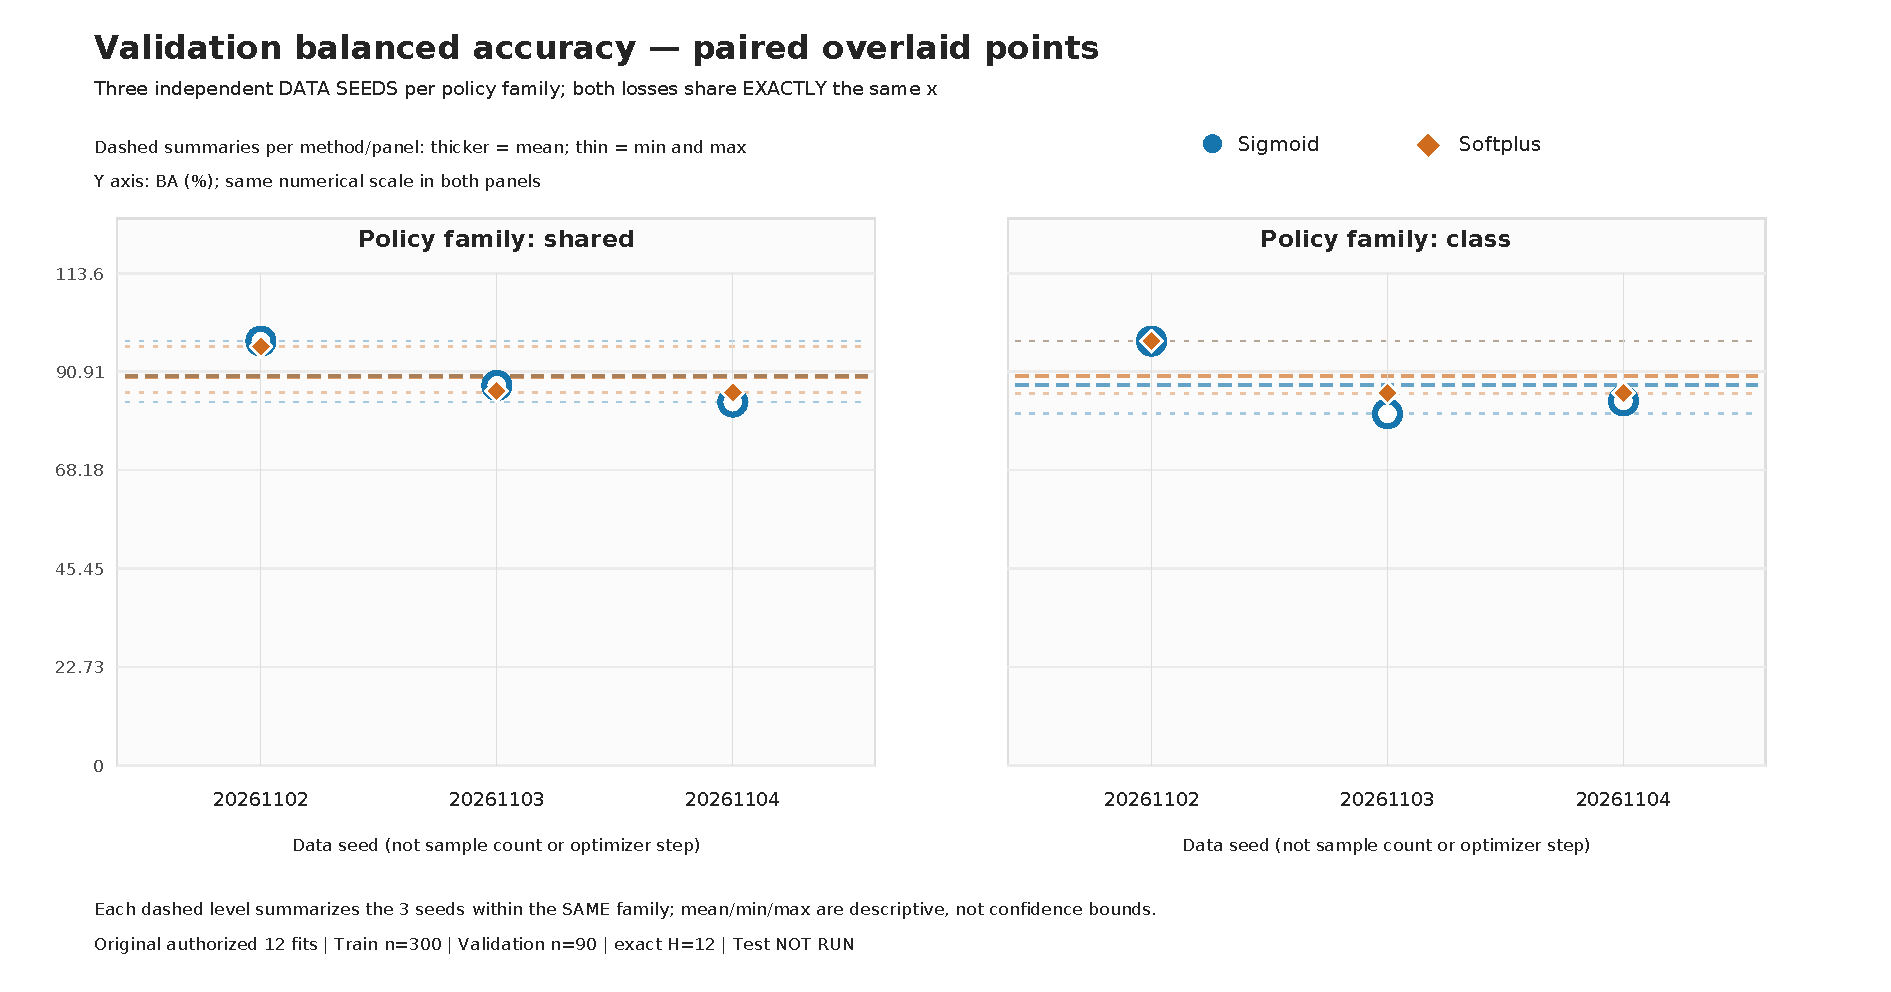
\includegraphics[width=0.98\linewidth]{code/experiments/ch4_loss_controlled_comparison/figures/phase2_tex/figure01_validation_BA_methods_by_seed.pdf}
\caption{دقت متوازن اعتبارسنجی در سه بذر مستقل، با مقایسه جفتی دو تابع زیان در هر بذر و خلاصه کمینه، میانگین و بیشینه برای هر خانواده سیاست. خطوط چین بازه اطمینان نیستند.}
\label{fig:ch4-e13-val-ba}
\end{figure}

\begin{figure}[htbp]
\centering
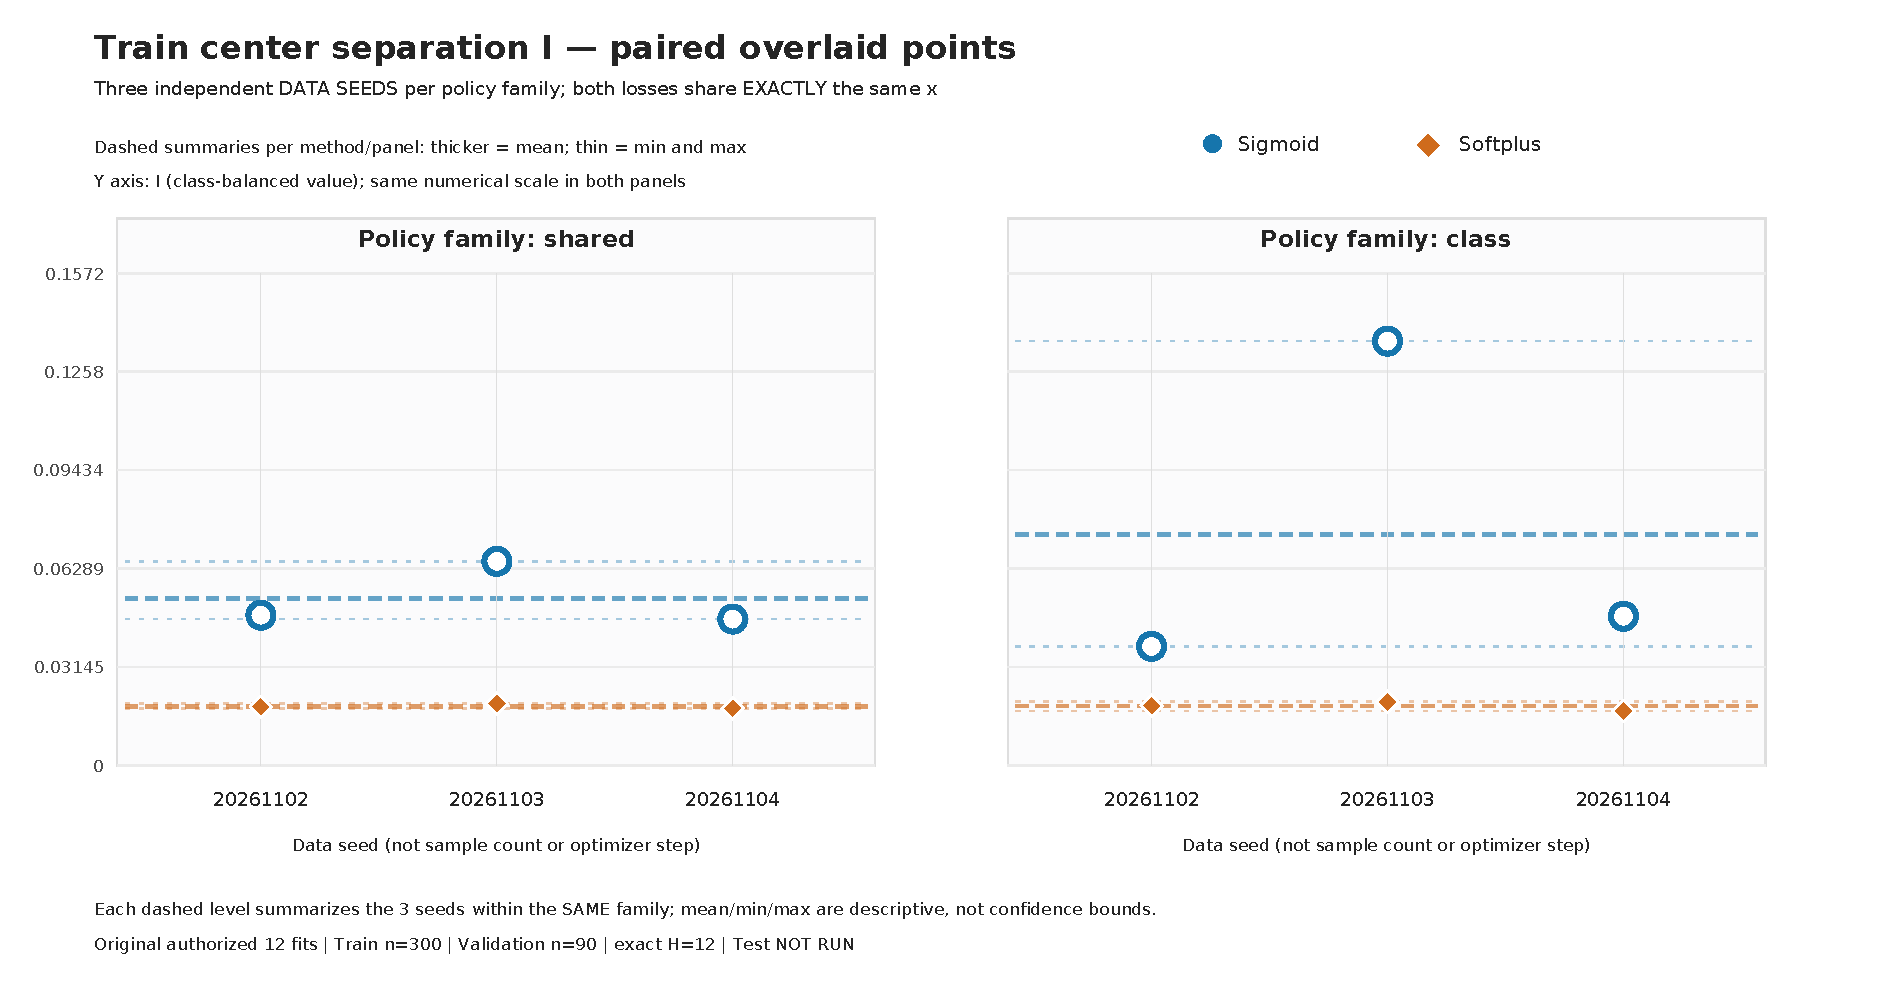
\includegraphics[width=0.98\linewidth]{code/experiments/ch4_loss_controlled_comparison/figures/phase2_tex/figure02_train_I_methods_by_seed.pdf}
\caption{جدایی مراکز آموزش در دو خانواده سیاست و سه بذر؛ مقدار معیار جدایی مراکز برای سیگموئید در همه شش جفت بیشتر است، بی‌آنکه بهبود دقت متوازن تضمین شود.}
\label{fig:ch4-e13-train-i}
\end{figure}
